% Copyright (c)  2005-2010 EDF-EADS-PHIMECA.
% Permission is granted to copy, distribute and/or modify this document
% under the terms of the GNU Free Documentation License, Version 1.2
% or any later version published by the Free Software Foundation;
% with no Invariant Sections, no Front-Cover Texts, and no Back-Cover
% Texts.  A copy of the license is included in the section entitled "GNU
% Free Documentation License".
\renewcommand{\filename}{docUC_InputWithData_LinearModel.tex}
\renewcommand{\filetitle}{UC : Building and validating a linear model from two samples}

% \HeaderNNIILevel
% \HeaderIILevel
\HeaderIIILevel


\index{Regression Linear Model!Factory}
\index{Regression Linear Model!Cloud sample - Line graph}
\index{Regression Linear Model!Residual graph}
\index{Regression Linear Model!Adjusted Rsquared test@Adjusted $R^2$ test}
\index{Regression Linear Model!Rsquared@$R^2$ test}
\index{Regression Linear Model!Fisher test}
\index{Regression Linear Model!Residual test}

\index{Graph!Regression linear model}
\index{Graph!Residual Regression linear model}
\index{Graph Manipulation!Bounding box}
\index{Graph Manipulation!ViewImage}
\index{Graph Manipulation!Show}



The objective of this Use Case is to build a linear regression model between a the scalar variable $Y$ and the n-dimensional one $\vect{X} = (X_i)_{i \leq n}$, as follows :
$$
\tilde{Y} = a_0 + \sum_i a_i X_i + \epsilon
$$
where $\epsilon$ is the residual, supposed to follow the Normal(0.0, 1.0) distribution.\\
Each coefficient $a_i$ is evaluated from both samples {\itshape Ysample} and {\itshape Xsample} and is accompagnied by a confidence interval and a p-value (which tests if they are significantly different from 0.0).\\




Details on the linear regression model  may be found in the Reference Guide (\href{OpenTURNS_ReferenceGuide.pdf}{see file Reference Guide - Step B -- Linear regression}).\\

Details on each object may be found in the User Manual  (\href{OpenTURNS_UserManual_TUI.pdf}{see User Manual - Statistics on sample / Fitting Test and Statistics on sample / Linear model}).\\


The linear model may be used to evaluate predictions on particular sample of the variable $X$ :  {\itshape particularXSample}.\\

The linear model may be validated :
\begin{itemize}
\item  graphically if {\itshape Xsample}  is of dimension 1, by drawing on the same graph the cloud ({\itshape Xsample, Ysample}) and the regression line, with the Open TURNS method {\itshape DrawLinearModelVisualTest},
\item  numerically with the following Open TURNS tests :
  \begin{itemize}
  \item {\itshape LinearModelRSquared} Test which tests the quality of the linear regression model. It evaluates the indicator $R^2$ (regression variance analysis) and compares it to a level,
  \item {\itshape LinearModelRAdjustedSquared} which  tests the quality of the linear regression model. It evaluates the indicator $R^2$ adjusted (regression variance analysis) and compares it to a level,
  \item {\itshape LinearModelFisher} Test which tests the nullity of the regression linear model coefficients (Fisher distribution used),
  \item {\itshape LinearModelResidualMean} Test which tests, under the hypothesis of a gaussian sample, if the mean of the residual is equal to zero. It is based on the Student test (equality of mean for two gaussian samples).
  \end{itemize}
\end{itemize}

The hypothesis on the residuals (centered gaussian distribution) may be validated :
\begin{itemize}
\item  graphically if {\itshape Xsample} is of dimension 1, by drawing the residual couples ($\epsilon_i, \epsilon_{i+1}$), where the residual $\epsilon_i$ is evaluated on the samples  ({\itshape Xsample, Ysample}) : $\epsilon_i = Ysample_i - \tilde{Y}_i$ with $\tilde{Y}_i = a_0 + a_1 Xsample_i$. The Open TURNS method is {\itshape DrawLinearModelResidualtest} ,
\item  numerically with the {\itshape LinearModelResidualMean} Test which tests, under the hypothesis of a gaussian sample, if the mean of the residual is equal to zero. It is based on the Student test (equality of mean for two gaussian samples).
\end{itemize}

\longrequirements{
  \begin{description}
  \item[$\bullet$] a 1D-sample : {\itshape Ysample}
  \item[type:]  NumericalSample
  \item[$\bullet$] a nD-sample : {\itshape Xsample}
  \item[type:]  NumericalSample
  \item[$\bullet$] a nD-sample : {\itshape particularXSample}
  \item[type:]  NumericalSample
  \end{description}
}
{
  \begin{description}
  \item[$\bullet$] a linear regression model : {\itshape linearRegressionModel}
  \item[type:]  LinearModel
  \item[$\bullet$] the linear coefficients $(a_i)_{0 \leq i \leq n}$ : {\itshape coefValues}
  \item[type:] scalarCollection
  \item[$\bullet$] the confidence intervals of each coefficient $a_i$
  \item[type:]  ConfidenceIntervalCollectionf
  \item[$\bullet$] the p-values of each coefficient $a_i$
  \item[type:]  ConfidenceIntervalCollection
  \item[$\bullet$] the predicted value on a particular sample : {\itshape predictedSample}
  \item[type:] NumericalSample
  \item[$\bullet$] the sample of resual values: {\itshape residualSample}
  \item[type:] NumericalSample
  \item[$\bullet$] the graph superposing the samples cloud and the regression line (in case of dimension 1 for X) : {\itshape linearRegressionModel.png, linearRegressionModel.eps}
  \item[type:]  files at format PNG or EPS or FIG
  \item[$\bullet$] the graph of residual values : {\itshape residualGraph.png, residualGraph.eps}
  \item[type:]  files at format PNG or EPS or FIG
  \item[$\bullet$] LinearModelRAdjustedSquared test result : {\itshape resultLinearModelRAdjustedSquared}
  \item[type:] TestResult
  \item[$\bullet$] LinearModelRSquared test result : {\itshape resultLinearModelRSquared}
  \item[type:] TestResult
  \item[$\bullet$] LinearModelFisher test result : {\itshape resultLinearModelFisher}
  \item[type:] TestResult
  \item[$\bullet$] LinearModelResidualMean test result : {\itshape resultLinearModelResidualMean}
  \item[type:] TestResult
  \end{description}
}

\textspace\\
Python script for this UseCase :

\begin{lstlisting}
  # Create the linear model from both sample : Ysample function of Xsample
  # CARE : Xsample is of dimension n and Ysample of dimension 1
  # The level confidence to evaluate the confidence interval is set to 0.90
  linearRegressionModel = LinearModelFactory().build(Xsample, Ysample, 0.90)

  # Get the coefficients ai
  print "coefficients of the linear regression model = " , linearRegressionModel.getRegression()

  # Get the confidence intervals of the ai coefficients
  print "confidence intervals of the coefficients = " , linearRegressionModel.getConfidenceIntervals()

  # Get the p values of the (n+1) coefficients ai:
  print "p-value of each coefficient = " , linearRegressionModel.getPValues()

  # Evaluate the predictions on the sample particularXSample
  print "predicted values on particularXSample = " , linearRegressionModel.getPredict(particularXSample)

  # Get the residuals
  print "residuals values = " , linearRegressionModel.getResidual(Xsample, Ysample)

  # GRAPH 1 : Validate the model with a visual test :
  # superposition of clouds (Xsample, Ysample)
  # ONLY if Xsample is a SCALAR numerical sample
  # + linear regression model
  # Create the graph structure
  linearRegressionGraph =  VisualTest.DrawLinearModel(Xsample, Ysample, linearRegressionModel)

  # Impose a bounding box : x-range and y-range
  # boundingBox = [xmin, xmax, ymin, ymax]
  myBoundingBox = NumericalPoint( (xmin, xmax, ymin, ymax) )
  linearRegressionGraph.setBoundingBox(myBoundingBox)

  # In order to see the graph without creating the associated files
  Show(linearRegressionGraph)

  # Draw the graph on the file linearRegressionModel.png and linearRegressionModel.eps
  # if the file adress is not fulfilled, the file is created in the current directory
  linearRegressionGraph.draw("linearRegressionModel")

  # View the bitmap file
  ViewImage(linearRegressionGraph.getBitmap())

  # Check if it worked
  print "bitmap = " , linearRegressionGraph.getBitmap()
  print "postscript = " , linearRegressionGraph.getPostscript()

  # GRAPH 2 : Draw the graph of the residual values
  # couples (residual i, residual i+1)
  # ONLY if Xsample is a SCALAR numerical sample
  # Create the graph structure
  residualValuesGraph = VisualTest.DrawLinearModelResidual(Xsample, Ysample, linearRegressionModel)

  # Impose a bounding box : x-range and y-range
  # boundingBox = [xmin, xmax, ymin, ymax]
  myBoundingBox = NumericalPoint( (xmin, xmax, ymin, ymax) )
  linearRegressionGraph.setBoundingBox(myBoundingBox)

  # In order to see the graph without creating the associated files
  Show(residualValuesGraph)

  # Draw the graph on the file residualGraph.png and residualGraph.eps
  # if the file adress is not fulfilled, the file is created in the current directory
  residualValuesGraph.draw("residualGraph")

  # View the bitmap file
  ViewImage(residualValuesGraph.getBitmap())

  # Check if it worked
  print "bitmap = " , residualValuesGraph.getBitmap()
  print "postscript = " , residualValuesGraph.getPostscript()

  # LinearModelRSquared Test tests the quality of the linear regression model.
  # It evaluates the R^2 indicator (regression variance analysis)
  # and compares it to a level
  # H0 = R^2 > level
  # Test = True <=> R^2 > level
  # p-value threshold : level CARE : it is NOT a probability here!
  # p-value : R^2 CARE : it is NOT a probability here!
  # Test = True <=> p-value > p-value threshold

  # The two following tests must be equal :
  # Test 1 : We don't give the linear model which is evaluated and then tested
  resultLinearModelRSquared1 = LinearModelTest.LinearModelRSquared(sampleX, sampleY, 0.90)

  # Test 2 : We give the regression linear model evaluated previously
  resultLinearModelRSquared2 = LinearModelTest.LinearModelRSquared(sampleX, sampleY, linearRegressionModel, 0.90)

  # Print result of the LinearModelRSquared Test
  print "Test Succes ? ", (resultLinearModelRSquared1.getBinaryQualityMeasure()==1)

  # Get the p-value of the LinearModelRSquared Test
  # CARE : it is NOT a probability here! but the R^2 value
  print "p-value of the LinearModelRSquared Test = ", resultLinearModelRSquared1.getPValue()

  # Get the p-value threshold of the LinearModelRSquared Test
  # CARE : it is NOT a probability here! but the level=0.90 here
  print "p-value threshold = ", resultLinearModelRSquared1.getThreshold()


  #  LinearModelAdjustedRSquared Test tests the quality of the linear regression model.
  # It evaluates the adjusted R^2 indicator (regression variance analysis)
  # and compare it to a level
  # H0 = adjusted aR^2 > level
  # Test = True <=> adjusted R^2 > level
  # p-value threshold : level CARE : it is NOT a probability here!
  # p-value : adjusted R^2 CARE : it is NOT a probability here!
  # Test = True <=> p-value > p-value threshold

  # The two tests must be equal
  # We don't give the linear model which is evaluated and then tested
  resultLinearModelAdjustedRSquared1 = LinearModelTest.LinearModelAdjustedRSquared(sampleX, sampleY, 0.90)

  # We give the regression linear model evaluated previously
  resultLinearModelAdjustedRSquared2 = LinearModelTest.LinearModelAdjustedRSquared(sampleX, sampleY, linearRegressionModel, 0.90)

  # Print result of the LinearModelAdjustedRSquared Test
  print "Test Succes ? ", (resultLinearModelAdjustedRSquared1.getBinaryQualityMeasure()==1)

  # Get the p-value of the LinearModelAdjustedRSquared Test
  # CARE : it is NOT a probability here! but the R^2 value
  print "p-value of the LinearModelAdjustedRSquared Test = ", resultLinearModelAdjustedRSquared1.getPValue()

  # Get the p-value threshold of the LinearModelAdjustedRSquared Test
  # CARE : it is NOT a probability here! but the level=0.90 here
  print "p-value threshold = ", resultLinearModelAdjustedRSquared1.getThreshold()

  #  LinearModelFisher Test tests the nullity of the regression linear model coefficients (Fisher distribution used).
  # H0 = the linear relation coefficients are those evaluated by the linear regresion
  # Test = True <=> the linear relation coefficients are those evaluated by the linear regresion
  # p-value threshold : probability of the H0 reject zone : 1-0.90
  # p-value : probability (test variable decision > test variable decision evaluated on the samples)
  # Test = True <=> p-value > p-value threshold

  # The two tests must be equal
  # Test 1 : We don't give the linear model which is evaluated and then tested
  resultLinearModelFisher1 = LinearModelTest.LinearModelFisher(sampleX, sampleY, 0.90)

  # Test 2 : We give the regression linear model evaluated previously
  resultLinearModelFisher2 = LinearModelTest.LinearModelFisher(sampleX, sampleY, linearRegressionModel, 0.90)

  # Print result of the LinearModelFisher Test
  print "Test Succes ? ", (resultLinearModelFisher1.getBinaryQualityMeasure()==1)

  # Get the p-value of the  LinearModelFisherTest
  print "p-value of the LinearModelFisher Test = ", resultLinearModelFisher1.getPValue()

  # Get the p-value threshold of the LinearModelFisher Test
  print "p-value threshold = ", resultLinearModelFisher1.getThreshold()

  #  LinearModelResidualMean Test tests, under the hypothesis of a  gaussian sample, if the mean of the residual is equal to zero. It is based on the Student test (equality of mean for two gaussian samples).
  # H0 = the residuals have a mean equal to zero
  # Test = True <=> the residuals have a mean equal to zero
  # p-value threshold : probability of the H0 reject zone : 1-0.90
  # p-value : probability (test variable decision > test variable decision evaluated on the samples)
  # Test = True <=> p-value > p-value threshold

  # The two tests must be equal
  # Test 1 : We don't give the linear model which is evaluated and then tested
  resultLinearModelResidualMean1 = LinearModelTest.LinearModelResidualMean(sampleX, sampleY, 0.90)

  # Test 2 : We give the regression linear model evaluated previously
  resultLinearModelResidualMean2 = LinearModelTest.LinearModelResidualMean(sampleX, sampleY, linearRegressionModel, 0.90)

  # Print result of the LinearModelResidualMean Test
  print "Test Succes ? ", (resultLinearModelResidualMean1.getBinaryQualityMeasure()==1)

  # Get the p-value of the  LinearModelResidualMeanTest
  print "p-value of the LinearModelResidualMean Test = ", resultLinearModelResidualMean1.getPValue()

  # Get the p-value threshold of the LinearModelResidualMean Test
  print "p-value threshold = ", resultLinearModelResidualMean1.getThreshold()
\end{lstlisting}
\textspace\\



The following figures draw the regression model superposed on the samples cloud ({\itshape Xsample, Ysample}) of size $10^3$ and the residuals graph in both cases :
\begin{itemize}
\item where the regression model seems validated : Figures  \ref{LMGood} and \ref{LMResidualGood},
\item where the regression model doesn't seem to be validated (relation of kind $Y = X^2$) : Figures  \ref{LMWrong} and \ref{LMResidualWrong}.
\item where the regression model doesn't seem to be validated (relation of kind $Y = sin(X)$) : Figures  \ref{LMWrong2} and \ref{LMResidualWrong2}.
\end{itemize}


\begin{figure}[H]
  \begin{minipage}{8cm}
    \begin{center}
      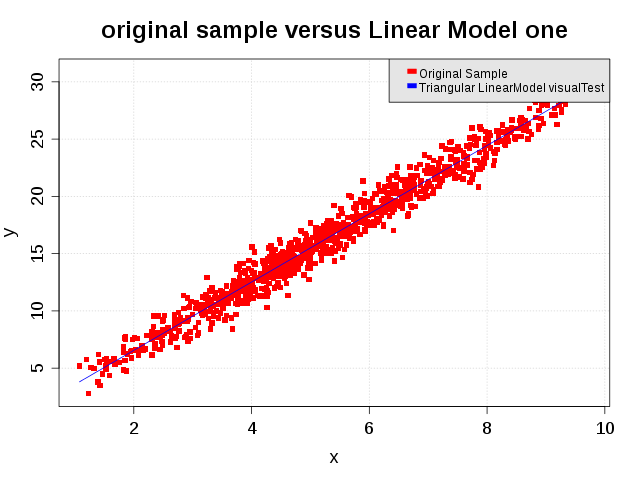
\includegraphics[width=8cm]{linearRegression_Graph.png}
      \caption{Visual validation of the Linear Regression Model.}
      \label{LMGood}
    \end{center}
  \end{minipage}
  \hfill
  \begin{minipage}{8cm}
    \begin{center}
      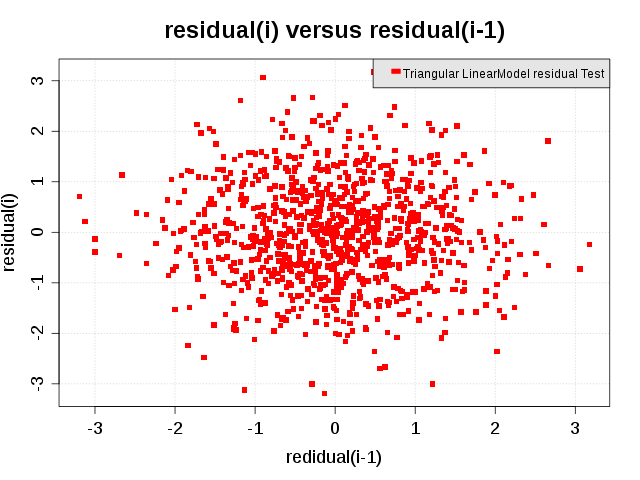
\includegraphics[width=8cm]{linearRegression_residualGraph.png}
      \caption{Visual validation of the Linear Regression Model : residuals graph.}
      \label{LMResidualGood}
    \end{center}
  \end{minipage}
\end{figure}



\begin{figure}[H]
  \begin{minipage}{8cm}
    \begin{center}
      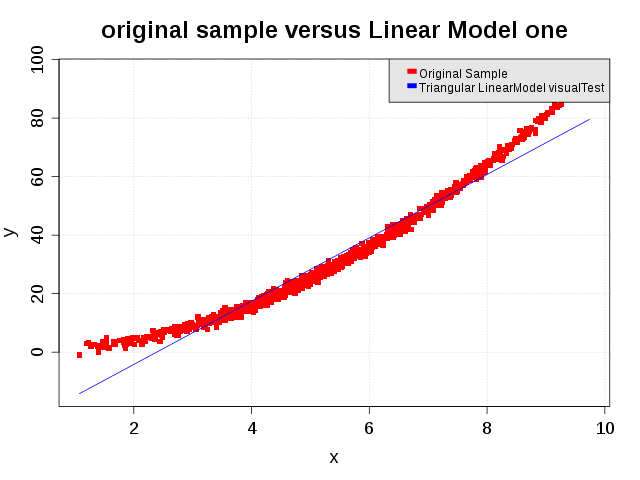
\includegraphics[width=8cm]{linearRegression_GraphWrong.png}
      \caption{Visual invalidation of the Linear Regression Model.}
      \label{LMWrong}
    \end{center}
  \end{minipage}
  \hfill
  \begin{minipage}{8cm}
    \begin{center}
      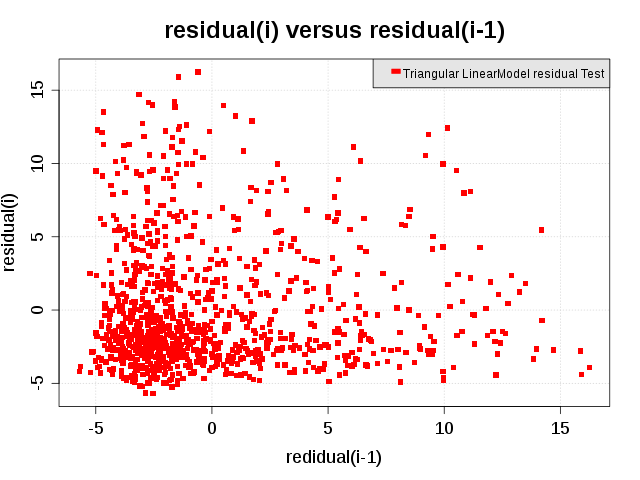
\includegraphics[width=8cm]{linearRegression_residualGraphWrong.png}
      \caption{Visual invalidation of the Linear Regression Model : residuals graph.}
      \label{LMResidualWrong}
    \end{center}
  \end{minipage}
\end{figure}


\begin{figure}[H]
  \begin{minipage}{8cm}
    \begin{center}
      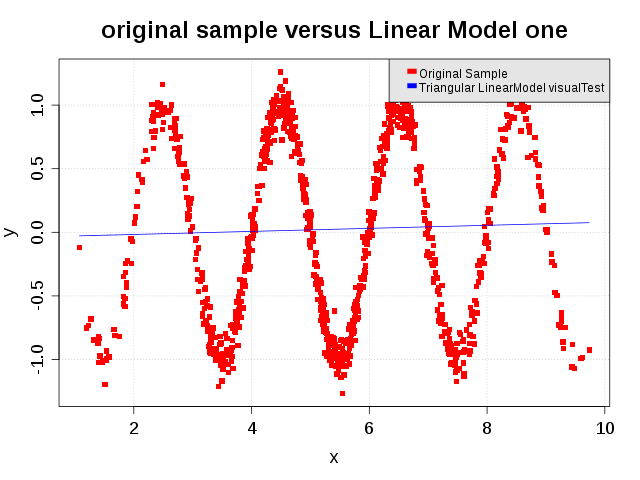
\includegraphics[width=8cm]{linearRegression_GraphWrong2.png}
      \caption{Visual invalidation of the Linear Regression Model.}
      \label{LMWrong2}
    \end{center}
  \end{minipage}
  \hfill
  \begin{minipage}{8cm}
    \begin{center}
      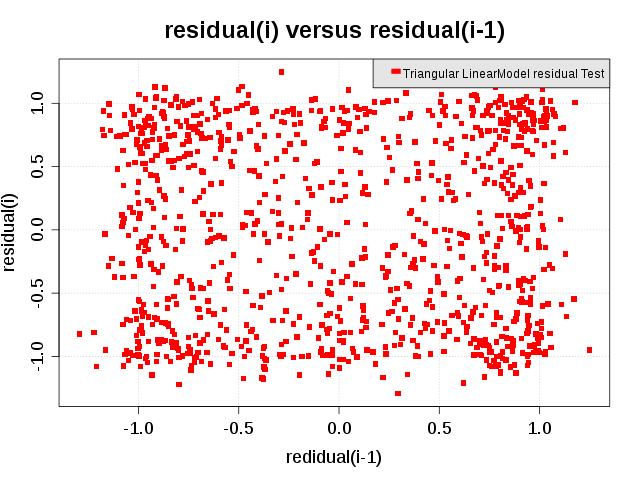
\includegraphics[width=8cm]{linearRegression_residualGraphWrong2.png}
      \caption{Visual invalidation of the Linear Regression Model : residuals graph.}
      \label{LMResidualWrong2}
    \end{center}
  \end{minipage}
\end{figure}


